%!TEX root = ../../Main.tex

\subsection{Задача 2}

Розглянемо також задачу:
%%%
\begin{equation}\label{eq:problem2}
\begin{cases}
	- \Delta u(x_1,x_2) + 10^5 u(x_1, x_2) = f(x_1,x_2), \\
	u|_\Gamma = 0 ,\\
	\Omega = \left[0;1\right] \times \left[0;1\right]
\end{cases}
\end{equation}
%%%

З точним розв'язком
%%
\begin{equation}
	u(x,y) = x_1^{14}x_2(1-x_1)(1-x_2)+x_1 x_2^{14}(1-x_1)(1-x_2),
\end{equation}
%
який зображений на \autoref{plot:problem2_exact}.
%%
\begin{figure}[H]
	\centering
    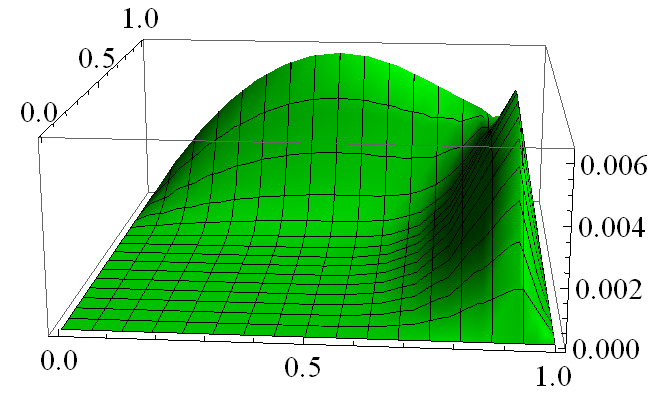
\includegraphics[scale=0.7]{problem2/ExactSolution}
    \captionsetup{format=hang,justification=centering}
    \caption{Точний розв'язок задачі \eqref{eq:problem2}. \newline $u(x_1,x_2) = (1-x_1)(1-x_2)x_1x_2(x_1^{13}+y_1^{13})$ }
    \label{plot:problem2_exact}
\end{figure}

Для адаптивної схеми задамо граничну точність в 7\%, а за початкове розбиття візьмемо рівномірне на сітці 7x7.


